\section{Data}
\label{sec:data}

We explore the behavior of the metrics on mock data with well-understood systematics as well as realistic mock data from past classification challenges.

Data is in the form of catalogs of posterior probability vectors $p(m \mid d)$ over $M$ classes $m$ conditioned on the observed data $d$, where one class is designated ``other'' to encompass never-before-seen classes, and each probability vector is normalized to sum to unity.
Such probabilities are more valuable than point estimates, which we call deterministic metrics in this work, because of their versatility in application and encapsulation of observational and systematic error that may propagate through inference (Roberts+17).

\subsection{Mock classifier systematics}
\label{sec:mockdata}

The test cases of this section are introduced to confirm that our metric aligns with our intuitive understanding of what constitutes a good classifier, that it should not reward classifications suffering from the systematics that we find most concerning.

For each, we will address:
\begin{enumerate}
  \item What defines this systematic?
  \item When has this systematic cropped up in the literature?
  \item What are our expectations for metric behavior?
\end{enumerate}

\aim{Anita Bahmanyar will write the descriptions of and motivation for the confusion matrix-based systematics tests, as well as how the data is generated (what the underlying functions from the notebook are doing).}

\aim{Let's condense these to a single multipanel figure.}

\begin{figure*}
	\begin{center}
		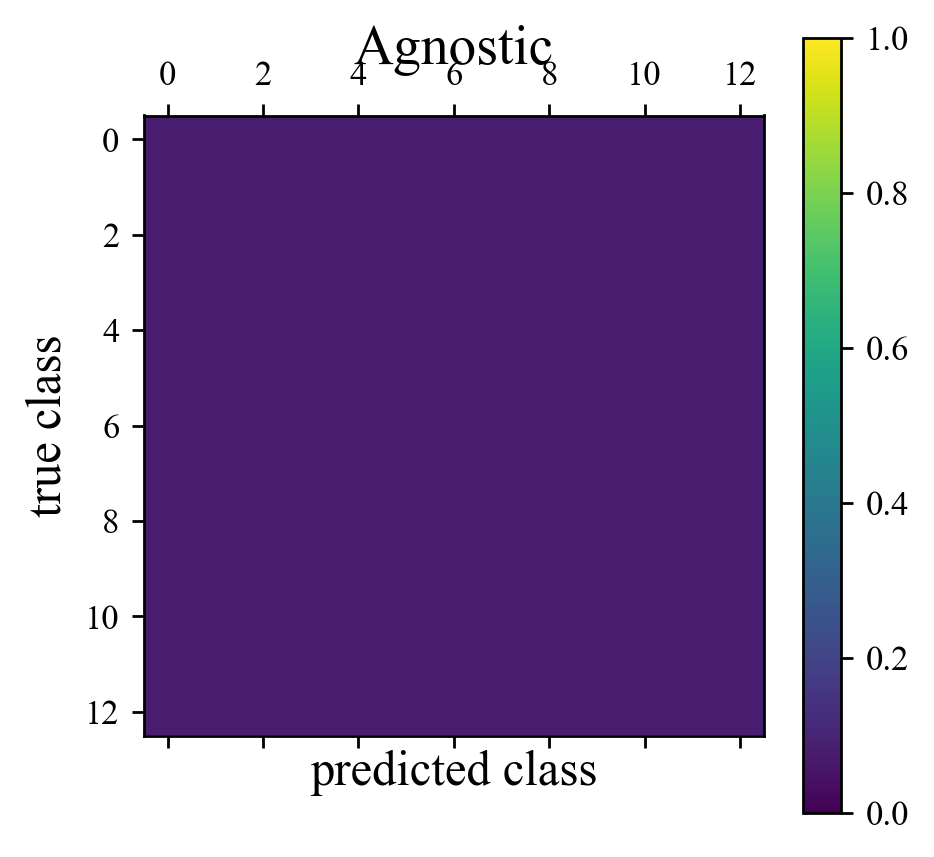
\includegraphics[width=0.2\textwidth]{./fig/Agnostic.png}
		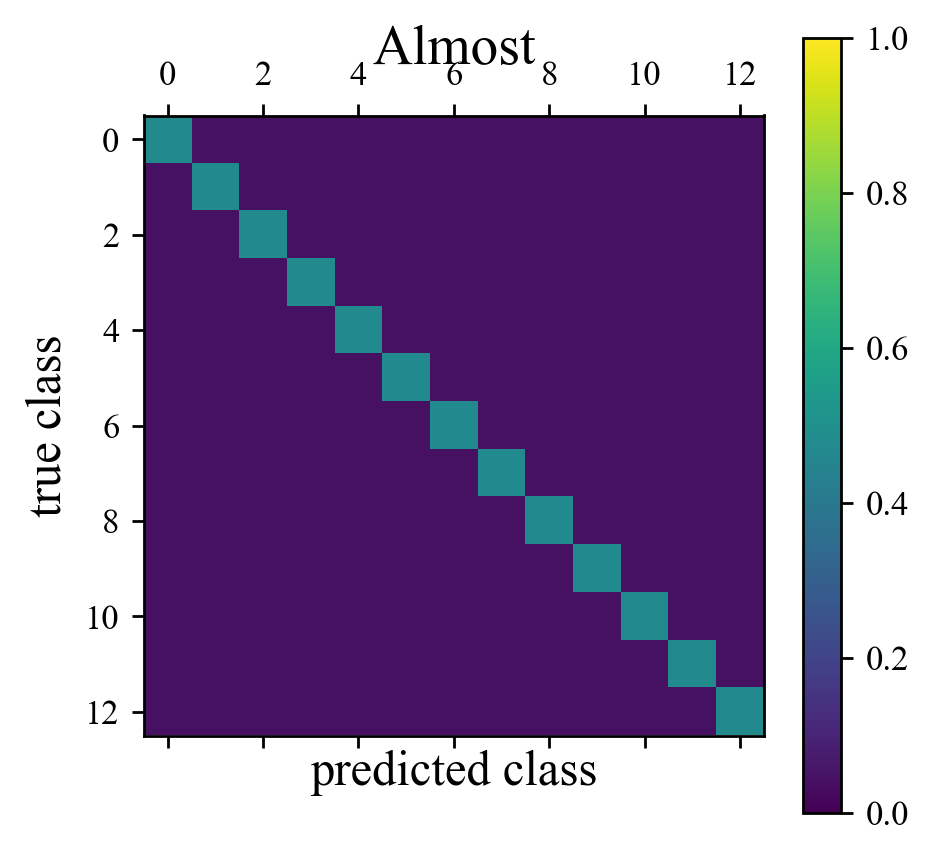
\includegraphics[width=0.2\textwidth]{./fig/Almost.png}
		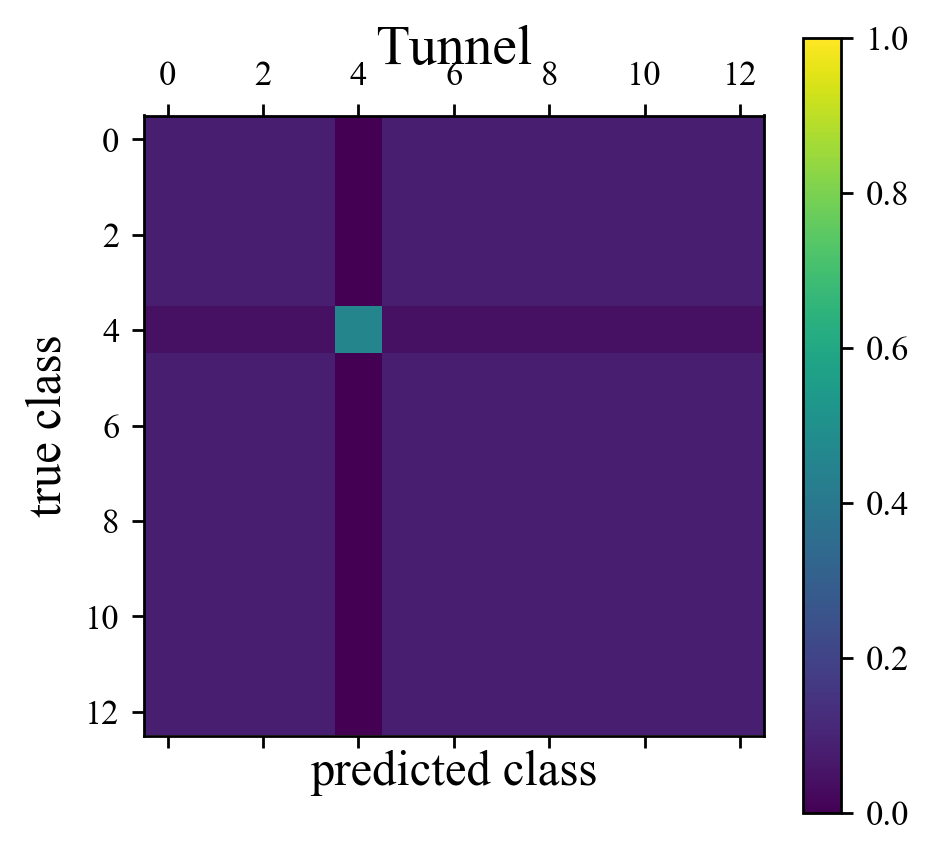
\includegraphics[width=0.2\textwidth]{./fig/Tunnel.png}
		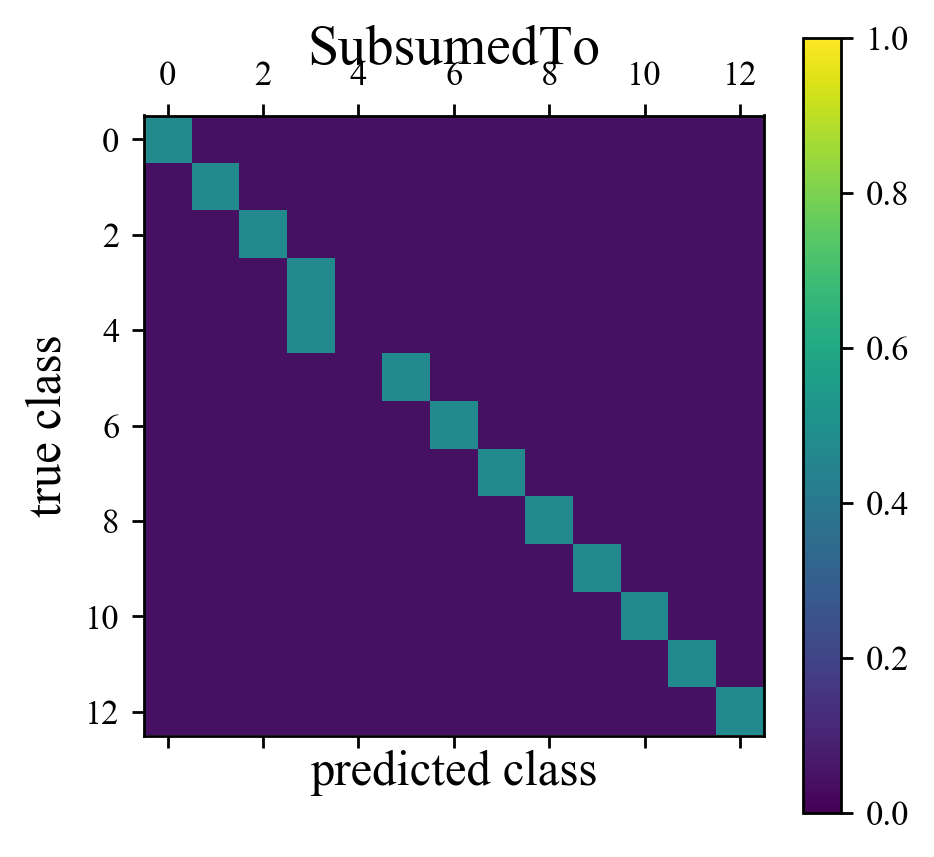
\includegraphics[width=0.2\textwidth]{./fig/SubsumedTo.png}\\
		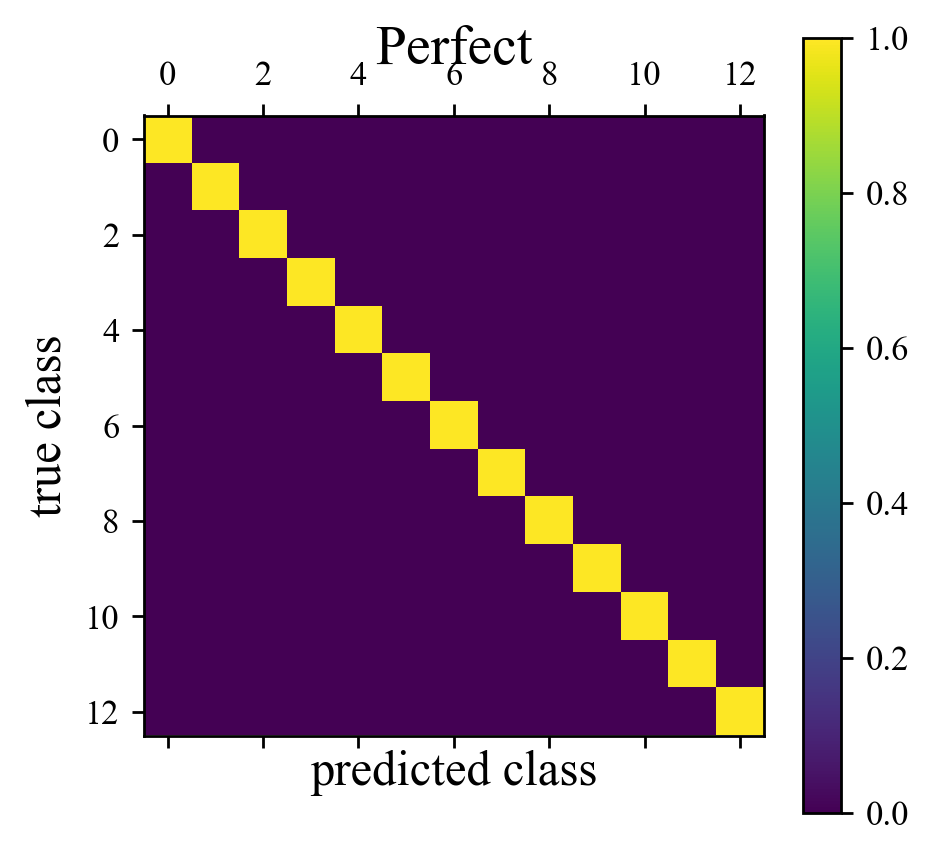
\includegraphics[width=0.2\textwidth]{./fig/Perfect.png}
		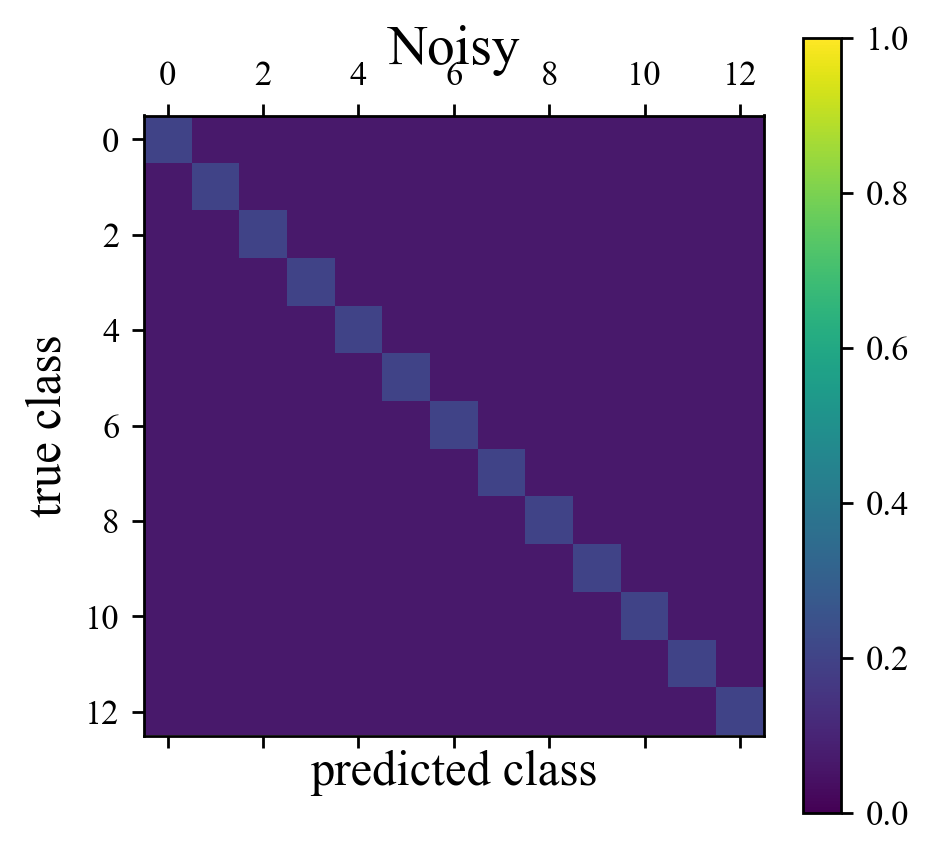
\includegraphics[width=0.2\textwidth]{./fig/Noisy.png}
		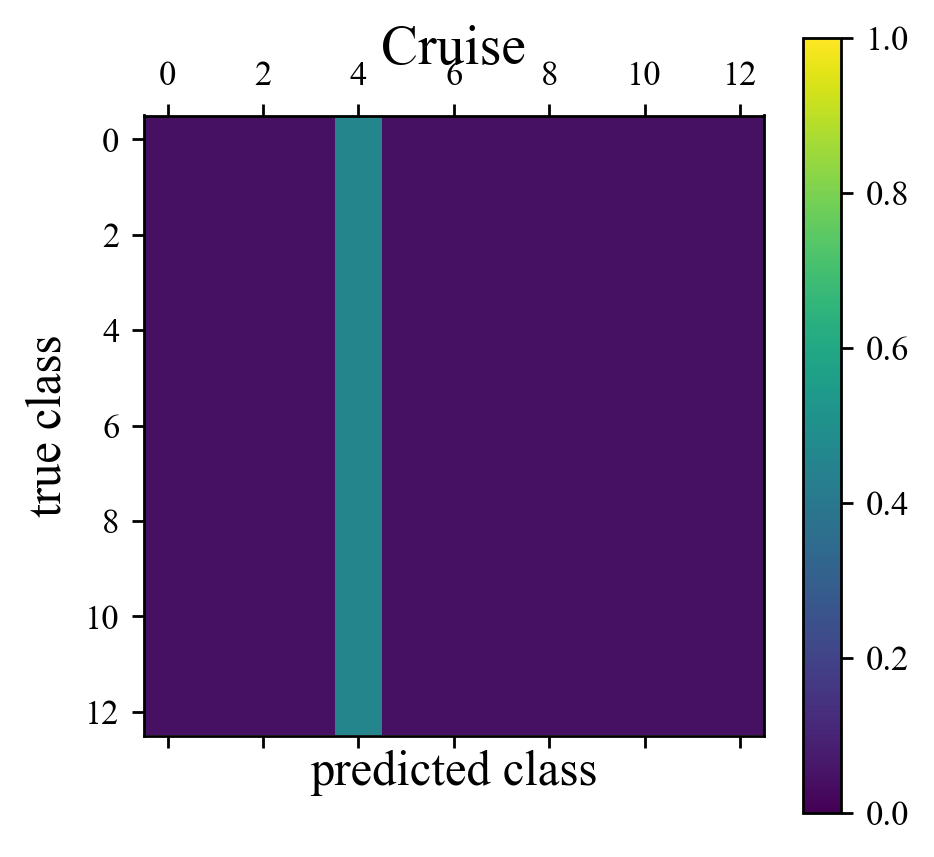
\includegraphics[width=0.2\textwidth]{./fig/Cruise.png}
		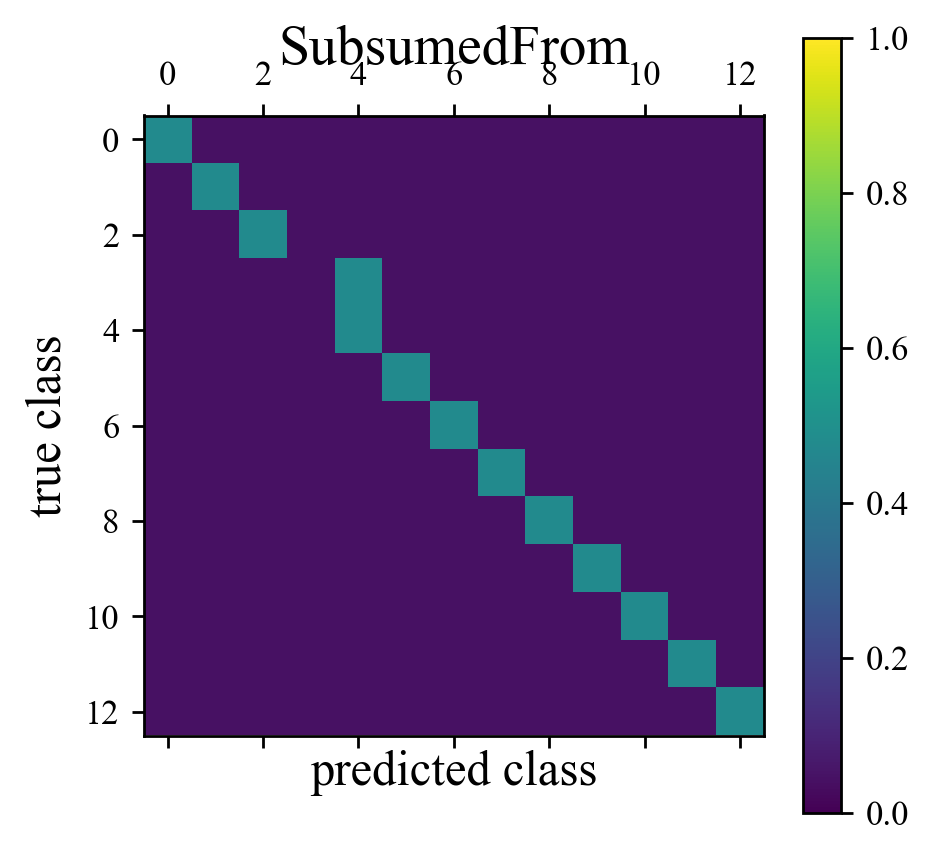
\includegraphics[width=0.2\textwidth]{./fig/SubsumedFrom.png}
		\caption{caption text for rightmost:
    top: upweight the predicted class encompassing both true classes, bottom: upweight the predicted class that is consistently misclassified}
		\label{fig:mock_cm}
	\end{center}
\end{figure*}

\subsubsection{Agnostic classifier}
\label{sec:agnostic_data}

uniform probabilities across all classes

\subsubsection{Perfect classifier}
\label{sec:perfect_data}

perfectly accurate on all classes

\subsubsection{Almost perfect classifier}
\label{sec:almost_data}

a slight perturbation of the perfect classifier

\subsubsection{Noisy classifier}
\label{sec:nois_datay}

a large perturbation of the perfect classifier

\subsubsection{Tunnel vision classifier}
\label{sec:tunnel_data}

classifies one class well and others randomly

\subsubsection{Cruise control classifier}
\label{sec:cruise_data}

classifies all objects as a single class

\subsubsection{Sumsuming classifier}
\label{sec:subsume_data}

consistently misclassifies one class as one other class

\subsection{Representative classifications and SNPhotCC}
\label{sec:realdata}

Classification problems in astronomy have historically focused on separating a heterogenous population into a limited number of subclasses (cite Kessler+2010), with the focus or goal being to identify one particular type of object.

In the Supernova Photometric Classification Challenge (SNPhotCC), the metric for deciding on who `won' the challenge was determined as a ratio of the efficiency of Type Ia classification and a `pseudo purity' factor, and a penalty for false-flagging (which is related to the cost of following up an object spectroscopically that is not a SNIa). The figure of metric was given by:

\begin{eqnarray}
\mathcal{C}_{FOM-Ia} &\equiv& \frac{1}{\mathcal{N}_{Ia}^{TOT}}\times \frac{(N_{Ia}^{\mathrm{true}})^2}{N_{Ia}^\mathrm{true}+W_{Ia}^\mathrm{false}N_{Ia}^\mathrm{false}}
\end{eqnarray}
%\aim{Renee Hlozek will write the descriptions of these datasets.}

The above reduces to $\mathcal{C}_{FOM-Ia}  = \epsilon_{Ia} + PP_{Ia},$ the efficiency and pseudopurity, which can be interpreted as the traditional purity factor in the limit that the weight $W_{Ia}^\mathrm{false} = 1$. For the SNPhotCC the false penalty was related to the size of the spectroscopic subsample as roughly $W_{Ia}^\mathrm{false} = 1 + \epsilon_{spec}^{-1} \gg 1$ but the conservative limit of $W_{Ia}^\mathrm{false} = 3$ was chosen to penalize wasted spectroscopic time over rejected SNe.

For future challenges, a more balanced metric can be used to ensure correct classifications across the range of objects, without focusing or highlighting a specific object as above.


\aim{We should also do this for Ashish's data in the form of confusion matrices.}

In response to the SNPhotCC, a range of classifications approaches were submitted, namely $\chi^{2}$ fits of the SN data to publicly available templates (ref. Nugent+), identification with the SiFTO light curve fitter (Conley et al. 2008) through the fitted values of the stretch, colour and also the $\chi^{2}$ of the fit for Ia fits, and a linear slope to magnitudes per day was used for the non-Ia sample. Other groups constructed a Hubble diagram from the training data, and used the residuals away from that Hubble diagram as a criterion for classification in the test data.

Other groups performed classification by reducing the dimensionality of the light curves (the so-called InCA approach). A general light curve shape (rather than one motivated by the physical differences between SNeIa and core collapse SNe) was assumed by some competitors and then a kernel density estimation was performed over the fit parameters, with various approaches employed including boosting over the feature space.


Machine learning was also eployed over the reduced data set of light-curve slopes (in magnitudes per day) as above to produce a predictive model for the training data. For more information on these methods and their success within the SNPhotCC, we refer the reader to Kessler+2010.

The above approaches vary between very physically motivated and \textbf{template based} (and also prone to bias given non-representativity of the test data) and agnostic and based on decomposition of the light curves into \textbf{generic features} (but also making use of less information in the classifications).
In figure~\ref{fig:snphotcc_cm} we show a range of classification approaches over the wavelet (feature) space (top row) and using templates (bottom row).

\subsubsection{SNPhotCC}
\label{sec:snphotcc}

\begin{figure*}
	\begin{center}
		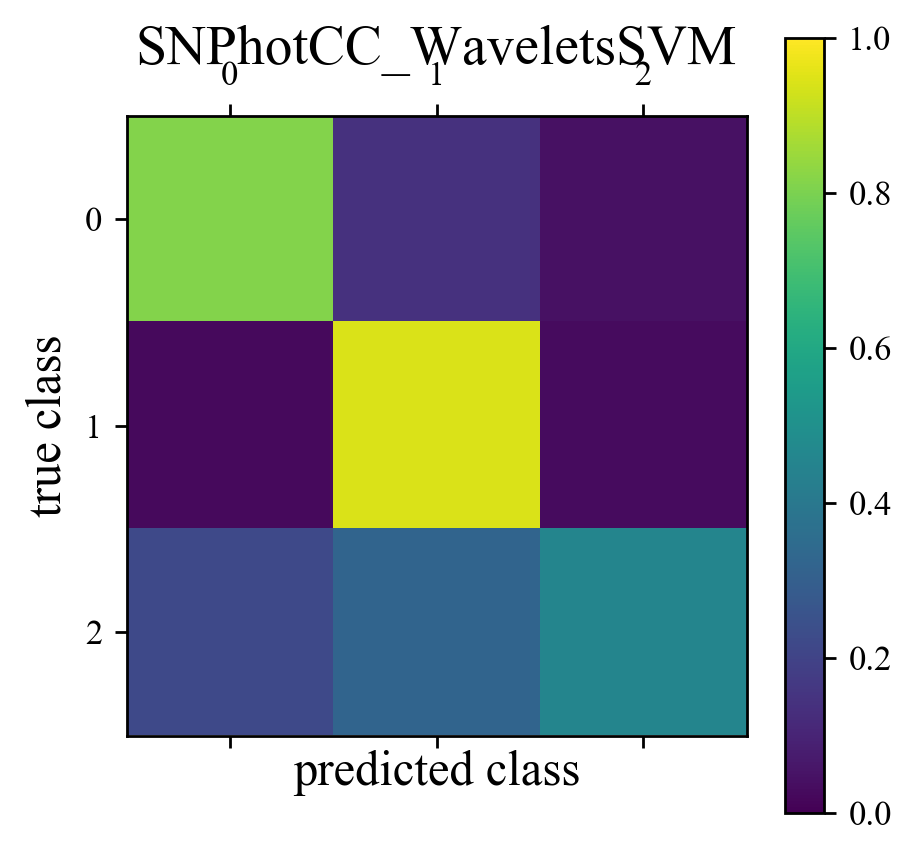
\includegraphics[width=0.2\textwidth]{./fig/SNPhotCC_WaveletsSVM_cm.png}
		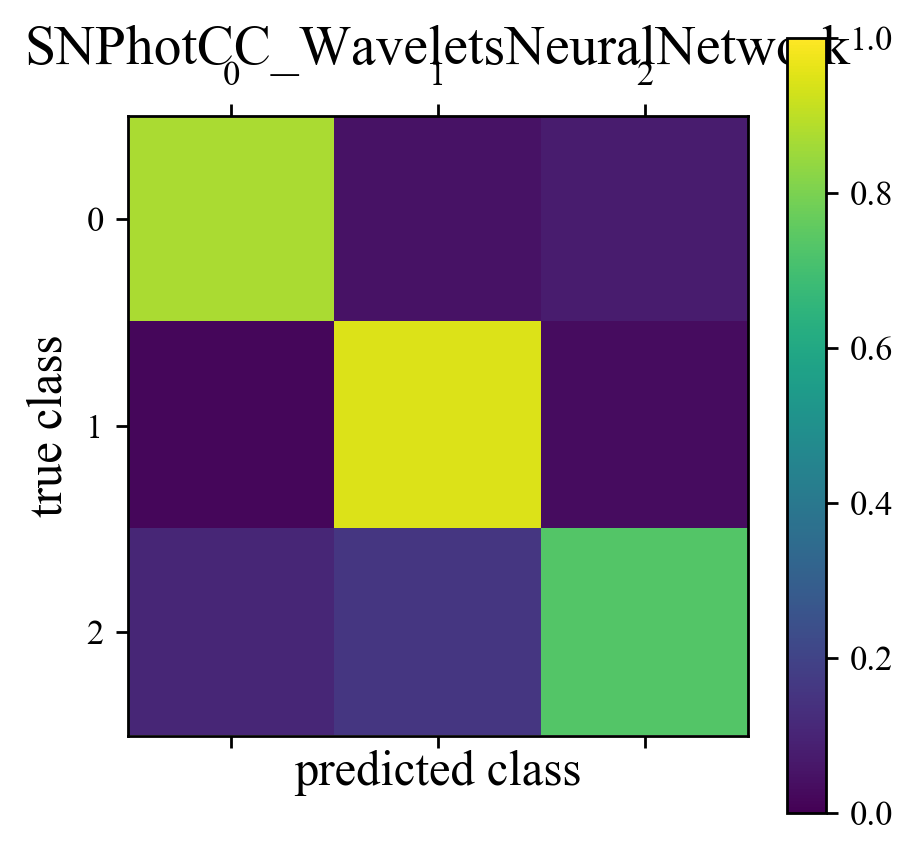
\includegraphics[width=0.2\textwidth]{./fig/SNPhotCC_WaveletsNeuralNetwork_cm.png}
		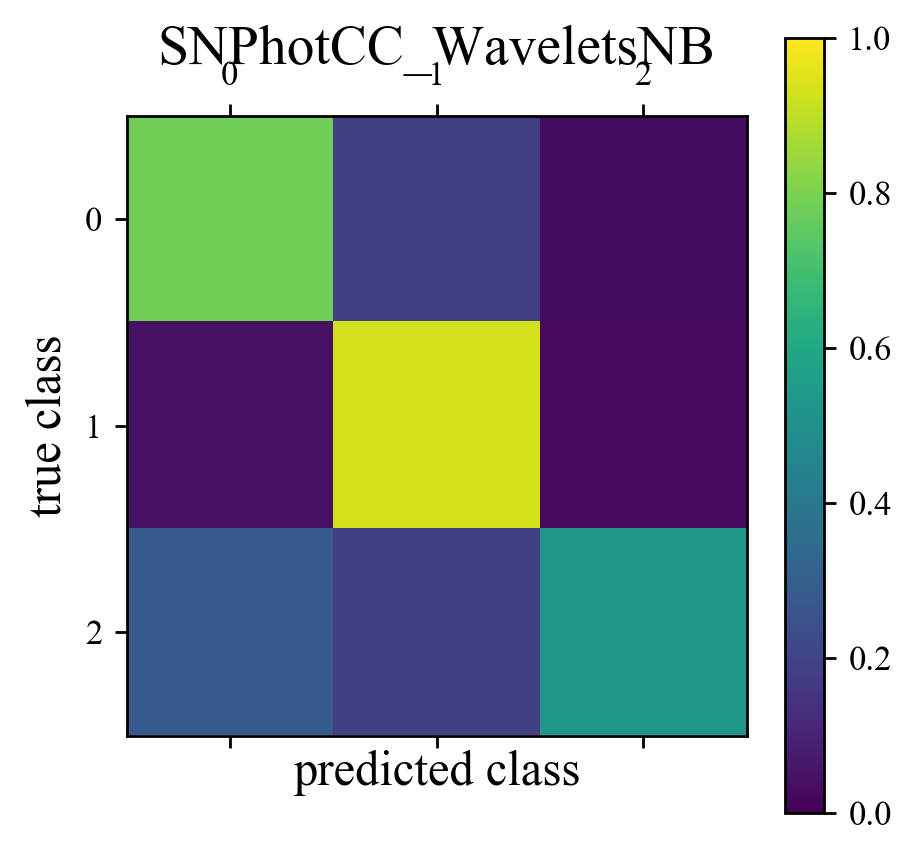
\includegraphics[width=0.2\textwidth]{./fig/SNPhotCC_WaveletsNB_cm.png}
		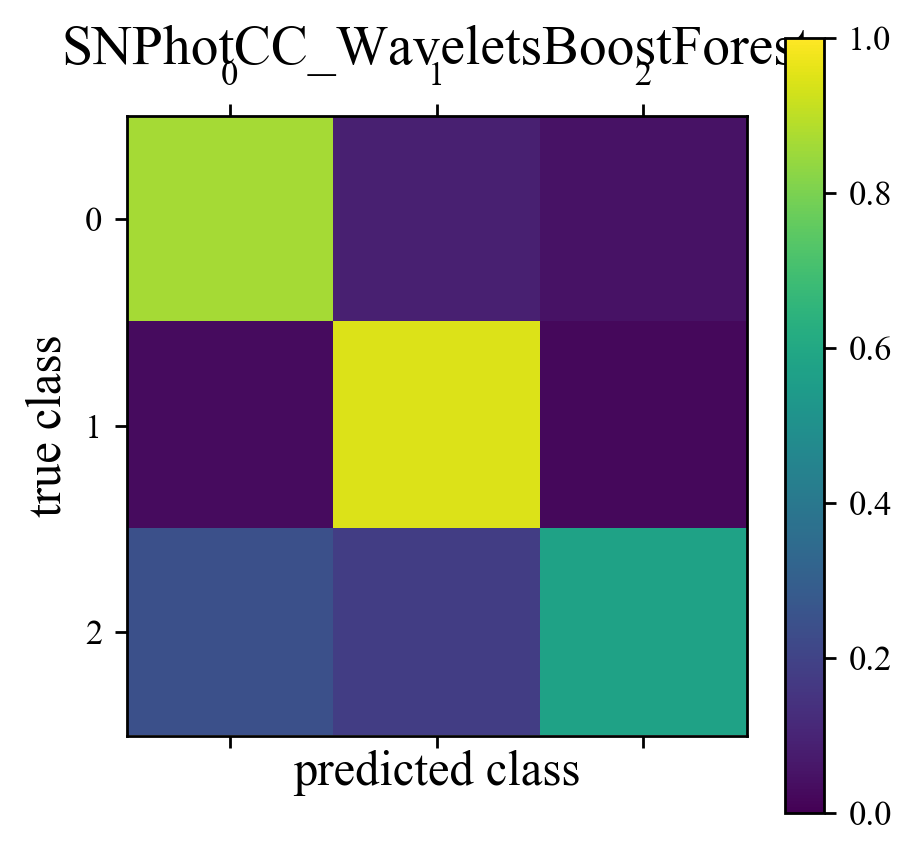
\includegraphics[width=0.2\textwidth]{./fig/SNPhotCC_WaveletsBoostForest_cm.png}\\
		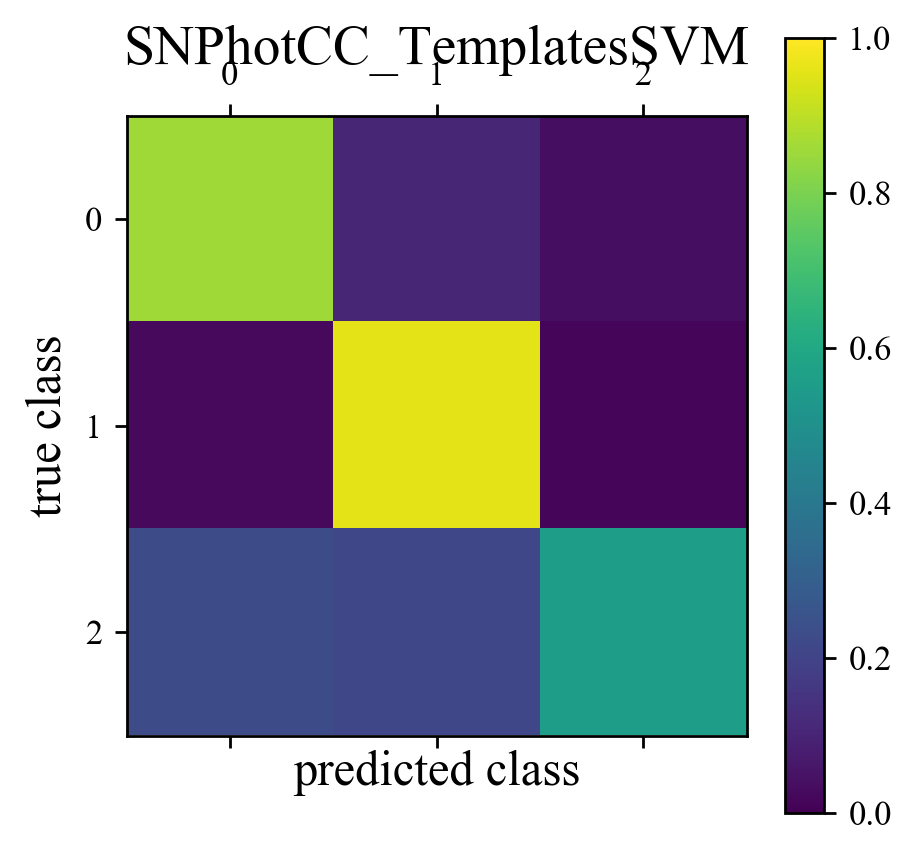
\includegraphics[width=0.2\textwidth]{./fig/SNPhotCC_TemplatesSVM_cm.png}
		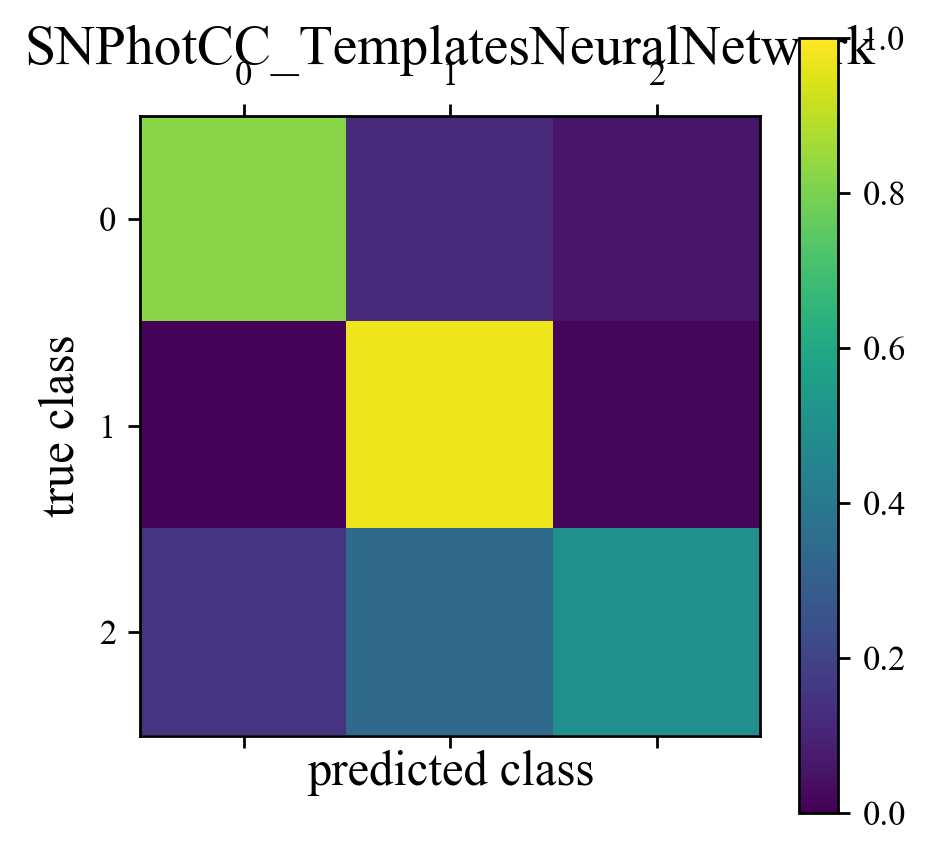
\includegraphics[width=0.2\textwidth]{./fig/SNPhotCC_TemplatesNeuralNetwork_cm.png}
		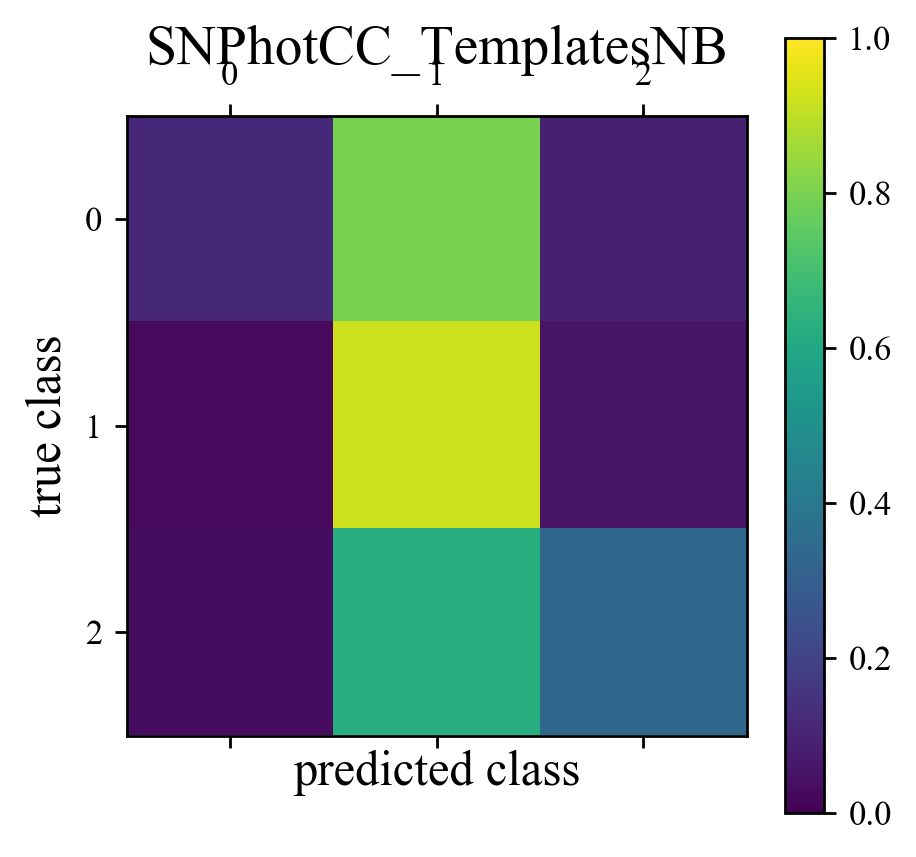
\includegraphics[width=0.2\textwidth]{./fig/SNPhotCC_TemplatesNB_cm.png}
		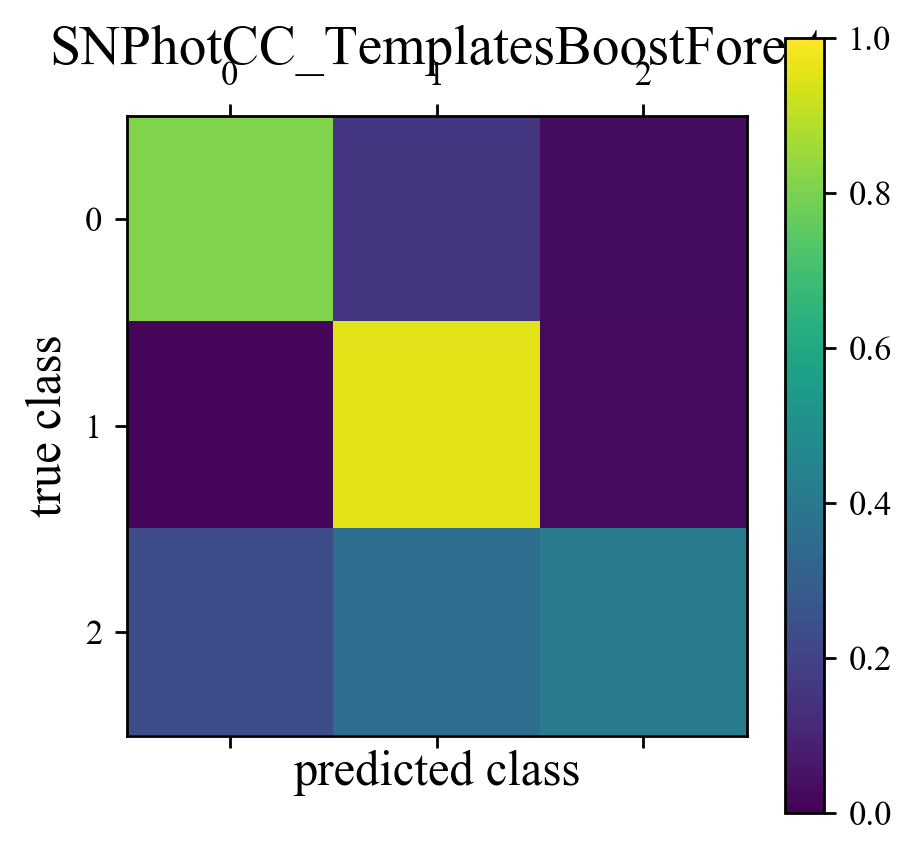
\includegraphics[width=0.2\textwidth]{./fig/SNPhotCC_TemplatesBoostForest_cm.png}
		\caption{\aim{Change confusion matrices to log-confusion matrices to better see contrast?}}
		\label{fig:snphotcc_cm}
	\end{center}
\end{figure*}

\subsubsection{Unknown dataset}
\label{sec:mystery}

\begin{figure*}
	\begin{center}
		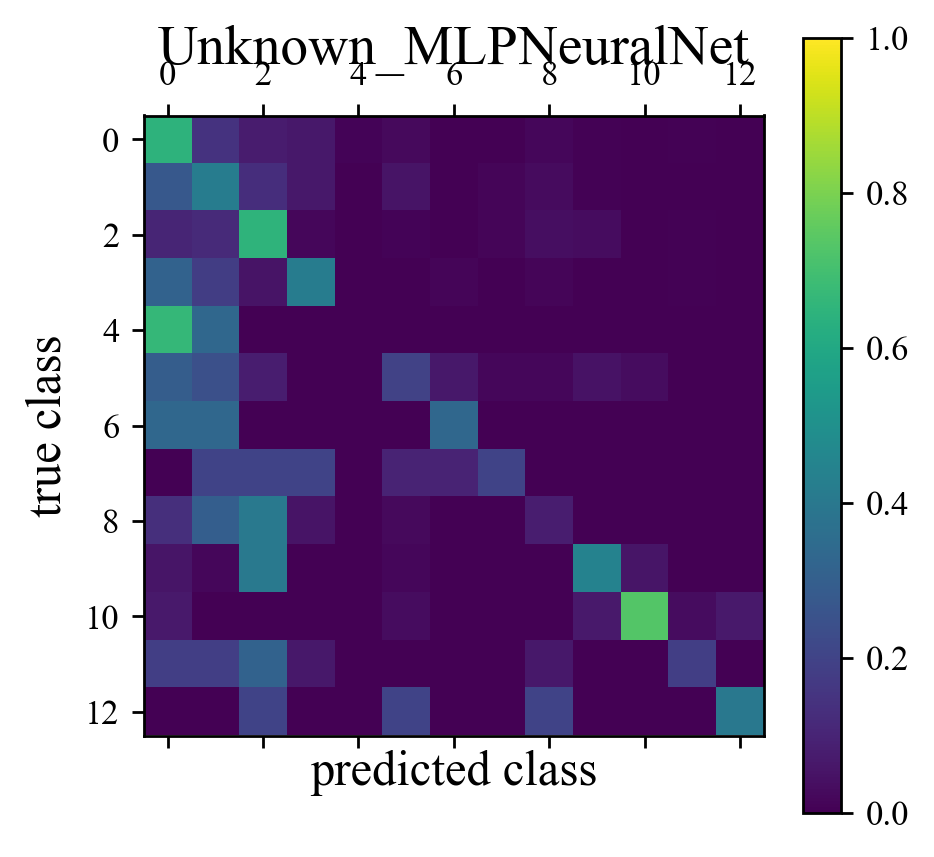
\includegraphics[width=0.3\textwidth]{./fig/Unknown_MLPNeuralNet_cm.png}
		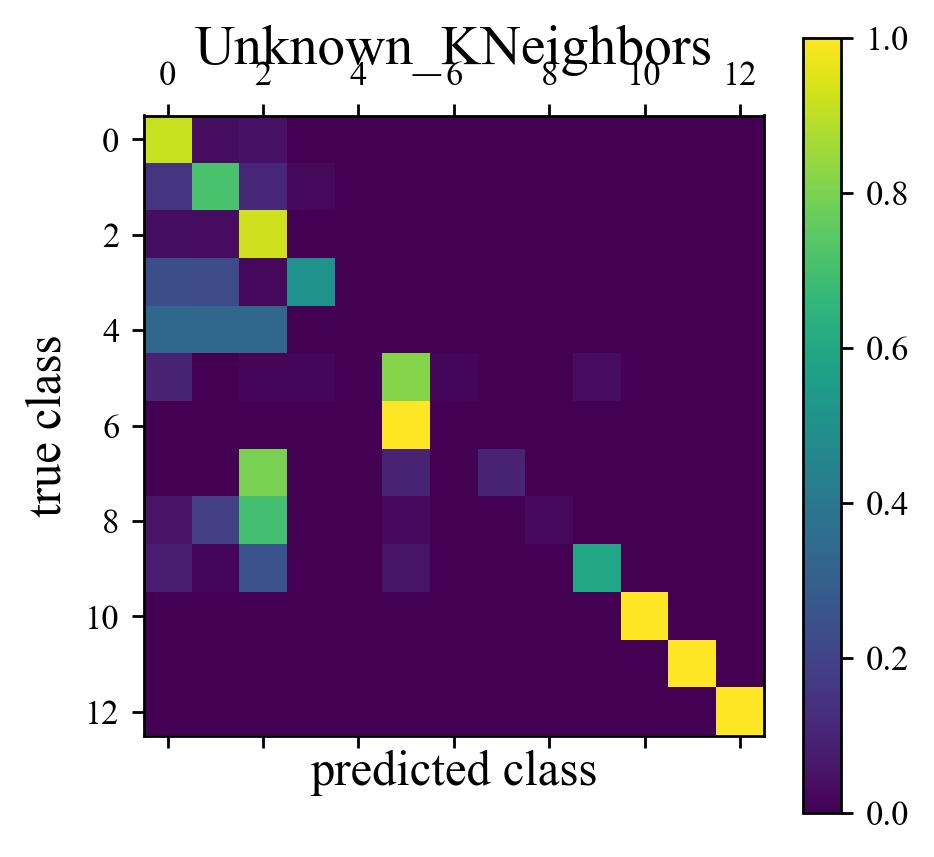
\includegraphics[width=0.3\textwidth]{./fig/Unknown_KNeighbors_cm.png}
		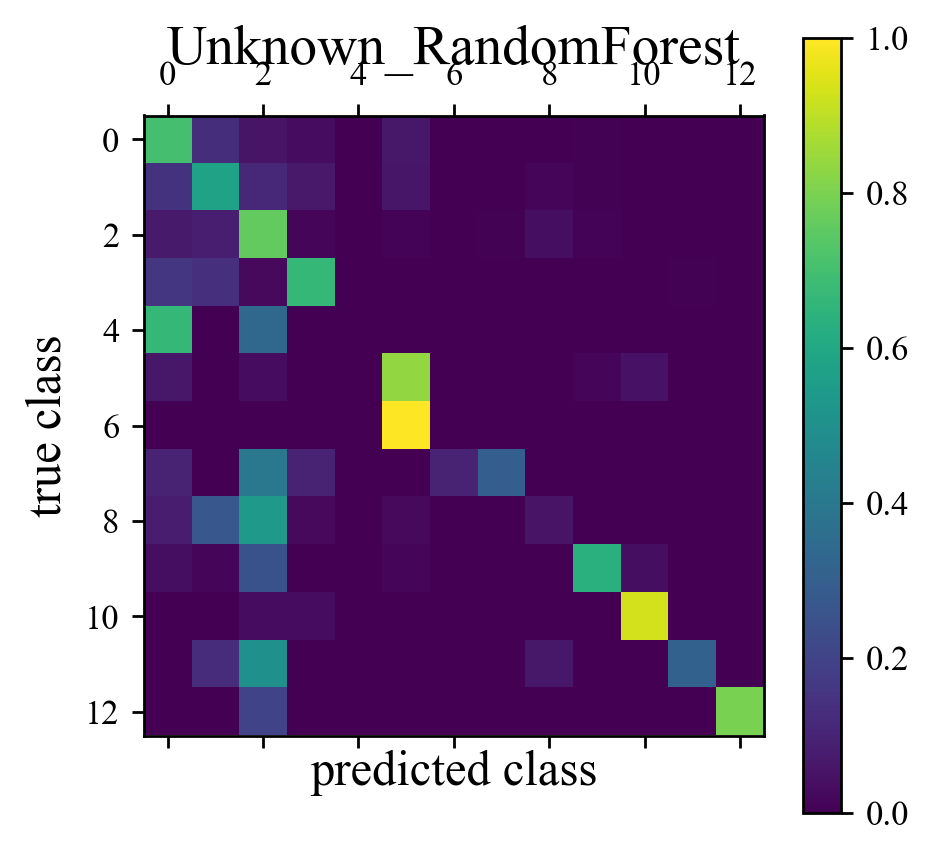
\includegraphics[width=0.3\textwidth]{./fig/Unknown_RandomForest_cm.png}
		\caption{}
		\label{fig:unknown_cm}
	\end{center}
\end{figure*}
